\documentclass{standalone}
\usepackage{tikz}
\usetikzlibrary{patterns, positioning}


\begin{document}
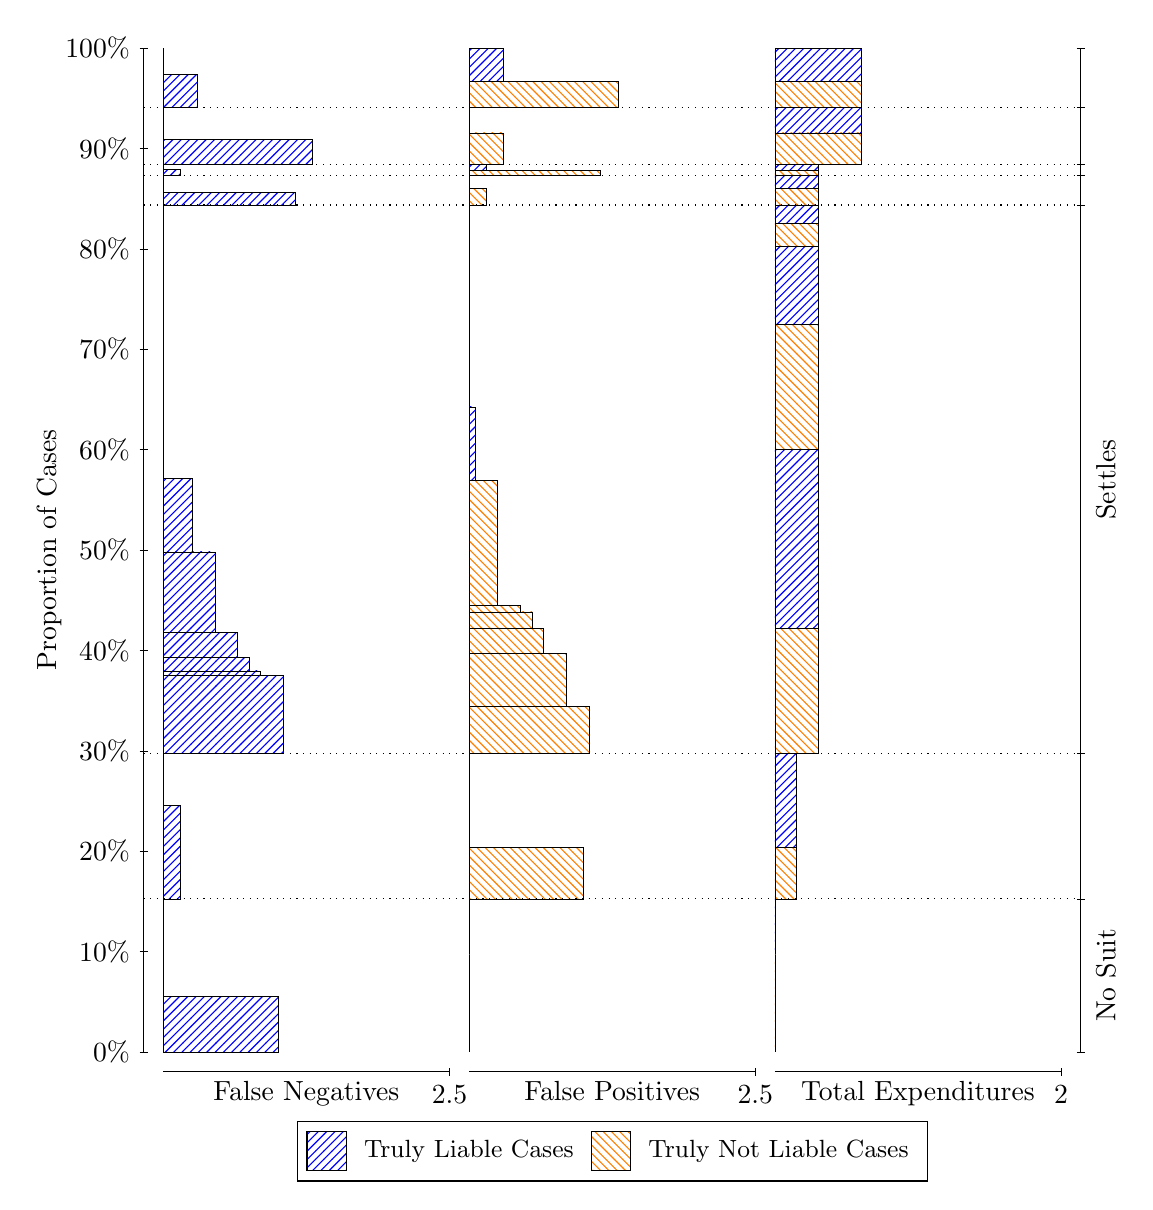
\begin{tikzpicture}
\draw[black, very thin] (1.5,1.75) -- (1.5,14.5);
\node[rotate=90, text=black, anchor=center] at (0.3, 8.125) {Proportion of Cases};
\draw[black, very thin] (1.45,1.75) -- (1.55,1.75);
\node[text=black, anchor=east] at (1.45, 1.75) {0\%};
\draw[black, very thin] (1.45,3.025) -- (1.55,3.025);
\node[text=black, anchor=east] at (1.45, 3.025) {10\%};
\draw[black, very thin] (1.45,4.3) -- (1.55,4.3);
\node[text=black, anchor=east] at (1.45, 4.3) {20\%};
\draw[black, very thin] (1.45,5.575) -- (1.55,5.575);
\node[text=black, anchor=east] at (1.45, 5.575) {30\%};
\draw[black, very thin] (1.45,6.85) -- (1.55,6.85);
\node[text=black, anchor=east] at (1.45, 6.85) {40\%};
\draw[black, very thin] (1.45,8.125) -- (1.55,8.125);
\node[text=black, anchor=east] at (1.45, 8.125) {50\%};
\draw[black, very thin] (1.45,9.4) -- (1.55,9.4);
\node[text=black, anchor=east] at (1.45, 9.4) {60\%};
\draw[black, very thin] (1.45,10.675) -- (1.55,10.675);
\node[text=black, anchor=east] at (1.45, 10.675) {70\%};
\draw[black, very thin] (1.45,11.95) -- (1.55,11.95);
\node[text=black, anchor=east] at (1.45, 11.95) {80\%};
\draw[black, very thin] (1.45,13.225) -- (1.55,13.225);
\node[text=black, anchor=east] at (1.45, 13.225) {90\%};
\draw[black, very thin] (1.45,14.5) -- (1.55,14.5);
\node[text=black, anchor=east] at (1.45, 14.5) {100\%};

\draw[black, very thin] (13.4,1.75) -- (13.4,14.5);
\draw[black, very thin] (13.35,1.75) -- (13.45,1.75);
\node[anchor=west] at (13.35, 1.75) {};
\draw[black, very thin] (13.35,3.6954) -- (13.45,3.6954);
\node[anchor=west] at (13.35, 3.6954) {};
\draw[black, very thin] (13.35,5.5378) -- (13.45,5.5378);
\node[anchor=west] at (13.35, 5.5378) {};
\draw[black, very thin] (13.35,12.507) -- (13.45,12.507);
\node[anchor=west] at (13.35, 12.507) {};
\draw[black, very thin] (13.35,12.882) -- (13.45,12.882);
\node[anchor=west] at (13.35, 12.882) {};
\draw[black, very thin] (13.35,13.024) -- (13.45,13.024);
\node[anchor=west] at (13.35, 13.024) {};
\draw[black, very thin] (13.35,13.742) -- (13.45,13.742);
\node[anchor=west] at (13.35, 13.742) {};
\draw[black, very thin] (13.35,14.5) -- (13.45,14.5);
\node[anchor=west] at (13.35, 14.5) {};

\draw[black, very thin, pattern color=blue, pattern=north east lines] (1.75,1.75) rectangle (3.2033,2.4561);
\draw[black, very thin, pattern color=orange, pattern=north west lines] (1.75,2.4561) rectangle (1.75,3.6954);
\draw[black, very thin, pattern color=blue, pattern=north east lines] (1.75,3.6954) rectangle (1.968,4.8807);
\draw[black, very thin, pattern color=orange, pattern=north west lines] (1.75,4.8807) rectangle (1.75,5.5378);
\draw[black, very thin, pattern color=blue, pattern=north east lines] (1.75,5.5378) rectangle (3.276,6.5281);
\draw[black, very thin, pattern color=blue, pattern=north east lines] (1.75,6.5281) rectangle (2.9853,6.5906);
\draw[black, very thin, pattern color=blue, pattern=north east lines] (1.75,6.5906) rectangle (2.84,6.7647);
\draw[black, very thin, pattern color=blue, pattern=north east lines] (1.75,6.7647) rectangle (2.6947,7.0805);
\draw[black, very thin, pattern color=blue, pattern=north east lines] (1.75,7.0805) rectangle (2.404,8.1015);
\draw[black, very thin, pattern color=blue, pattern=north east lines] (1.75,8.1015) rectangle (2.1133,9.0359);
\draw[black, very thin, pattern color=orange, pattern=north west lines] (1.75,9.0359) rectangle (1.75,12.507);
\draw[black, very thin, pattern color=blue, pattern=north east lines] (1.75,12.507) rectangle (3.4213,12.667);
\draw[black, very thin, pattern color=orange, pattern=north west lines] (1.75,12.667) rectangle (1.75,12.882);
\draw[black, very thin, pattern color=blue, pattern=north east lines] (1.75,12.882) rectangle (1.968,12.963);
\draw[black, very thin, pattern color=orange, pattern=north west lines] (1.75,12.963) rectangle (1.75,13.024);
\draw[black, very thin, pattern color=blue, pattern=north east lines] (1.75,13.024) rectangle (3.6393,13.344);
\draw[black, very thin, pattern color=orange, pattern=north west lines] (1.75,13.344) rectangle (1.75,13.742);
\draw[black, very thin, pattern color=blue, pattern=north east lines] (1.75,13.742) rectangle (2.186,14.166);
\draw[black, very thin, pattern color=orange, pattern=north west lines] (1.75,14.166) rectangle (1.75,14.5);
\draw[black, very thin, pattern color=orange, pattern=north west lines] (5.6333,1.75) rectangle (5.6333,2.9893);
\draw[black, very thin, pattern color=blue, pattern=north east lines] (5.6333,2.9893) rectangle (5.6333,3.6954);
\draw[black, very thin, pattern color=orange, pattern=north west lines] (5.6333,3.6954) rectangle (7.0867,4.3525);
\draw[black, very thin, pattern color=blue, pattern=north east lines] (5.6333,4.3525) rectangle (5.6333,5.5378);
\draw[black, very thin, pattern color=orange, pattern=north west lines] (5.6333,5.5378) rectangle (7.1593,6.1385);
\draw[black, very thin, pattern color=orange, pattern=north west lines] (5.6333,6.1385) rectangle (6.8687,6.8166);
\draw[black, very thin, pattern color=orange, pattern=north west lines] (5.6333,6.8166) rectangle (6.578,7.1276);
\draw[black, very thin, pattern color=orange, pattern=north west lines] (5.6333,7.1276) rectangle (6.4327,7.3403);
\draw[black, very thin, pattern color=orange, pattern=north west lines] (5.6333,7.3403) rectangle (6.2873,7.419);
\draw[black, very thin, pattern color=orange, pattern=north west lines] (5.6333,7.419) rectangle (5.9967,9.0085);
\draw[black, very thin, pattern color=blue, pattern=north east lines] (5.6333,9.0085) rectangle (5.706,9.9429);
\draw[black, very thin, pattern color=blue, pattern=north east lines] (5.6333,9.9429) rectangle (5.6333,12.507);
\draw[black, very thin, pattern color=orange, pattern=north west lines] (5.6333,12.507) rectangle (5.8513,12.722);
\draw[black, very thin, pattern color=blue, pattern=north east lines] (5.6333,12.722) rectangle (5.6333,12.882);
\draw[black, very thin, pattern color=orange, pattern=north west lines] (5.6333,12.882) rectangle (7.3047,12.943);
\draw[black, very thin, pattern color=blue, pattern=north east lines] (5.6333,12.943) rectangle (5.8513,13.024);
\draw[black, very thin, pattern color=orange, pattern=north west lines] (5.6333,13.024) rectangle (6.0693,13.421);
\draw[black, very thin, pattern color=blue, pattern=north east lines] (5.6333,13.421) rectangle (5.6333,13.742);
\draw[black, very thin, pattern color=orange, pattern=north west lines] (5.6333,13.742) rectangle (7.5227,14.076);
\draw[black, very thin, pattern color=blue, pattern=north east lines] (5.6333,14.076) rectangle (6.0693,14.5);
\draw[black, very thin, pattern color=orange, pattern=north west lines] (9.5167,1.75) rectangle (9.5167,2.9893);
\draw[black, very thin, pattern color=blue, pattern=north east lines] (9.5167,2.9893) rectangle (9.5167,3.6954);
\draw[black, very thin, pattern color=orange, pattern=north west lines] (9.5167,3.6954) rectangle (9.7892,4.3525);
\draw[black, very thin, pattern color=blue, pattern=north east lines] (9.5167,4.3525) rectangle (9.7892,5.5378);
\draw[black, very thin, pattern color=orange, pattern=north west lines] (9.5167,5.5378) rectangle (10.062,7.1276);
\draw[black, very thin, pattern color=blue, pattern=north east lines] (9.5167,7.1276) rectangle (10.062,9.3987);
\draw[black, very thin, pattern color=orange, pattern=north west lines] (9.5167,9.3987) rectangle (10.062,10.988);
\draw[black, very thin, pattern color=blue, pattern=north east lines] (9.5167,10.988) rectangle (10.062,11.978);
\draw[black, very thin, pattern color=orange, pattern=north west lines] (9.5167,11.978) rectangle (10.062,12.27);
\draw[black, very thin, pattern color=blue, pattern=north east lines] (9.5167,12.27) rectangle (10.062,12.507);
\draw[black, very thin, pattern color=orange, pattern=north west lines] (9.5167,12.507) rectangle (10.062,12.722);
\draw[black, very thin, pattern color=blue, pattern=north east lines] (9.5167,12.722) rectangle (10.062,12.882);
\draw[black, very thin, pattern color=orange, pattern=north west lines] (9.5167,12.882) rectangle (10.062,12.943);
\draw[black, very thin, pattern color=blue, pattern=north east lines] (9.5167,12.943) rectangle (10.062,13.024);
\draw[black, very thin, pattern color=orange, pattern=north west lines] (9.5167,13.024) rectangle (10.607,13.421);
\draw[black, very thin, pattern color=blue, pattern=north east lines] (9.5167,13.421) rectangle (10.607,13.742);
\draw[black, very thin, pattern color=orange, pattern=north west lines] (9.5167,13.742) rectangle (10.607,14.076);
\draw[black, very thin, pattern color=blue, pattern=north east lines] (9.5167,14.076) rectangle (10.607,14.5);
\draw[black, dotted] (1.5,3.6954) -- (13.4,3.6954);
\draw[black, dotted] (1.5,5.5378) -- (13.4,5.5378);
\draw[black, dotted] (1.5,12.507) -- (13.4,12.507);
\draw[black, dotted] (1.5,12.882) -- (13.4,12.882);
\draw[black, dotted] (1.5,13.024) -- (13.4,13.024);
\draw[black, dotted] (1.5,13.742) -- (13.4,13.742);
\draw[black, very thin] (1.75,1.5) -- (5.3833,1.5);
\node[text=black, anchor=north] at (3.5667, 1.5) {False Negatives};
\draw[black, very thin] (5.3833,1.45) -- (5.3833,1.55);
\node[text=black, anchor=north] at (5.3833, 1.45) {2.5};

\draw[black, very thin] (5.6333,1.5) -- (9.2667,1.5);
\node[text=black, anchor=north] at (7.45, 1.5) {False Positives};
\draw[black, very thin] (9.2667,1.45) -- (9.2667,1.55);
\node[text=black, anchor=north] at (9.2667, 1.45) {2.5};

\draw[black, very thin] (9.5167,1.5) -- (13.15,1.5);
\node[text=black, anchor=north] at (11.333, 1.5) {Total Expenditures};
\draw[black, very thin] (13.15,1.45) -- (13.15,1.55);
\node[text=black, anchor=north] at (13.15, 1.45) {2};

\node[text=black, centered, rotate=90] at (13.72, 2.7227) {No Suit};

\node[text=black, centered, rotate=90] at (13.72, 9.0222) {Settles};





\draw (7.449999999999999,1.5) node[draw=none] (baseCoordinate) {};
\begin{scope}[align=center]
        \matrix[scale=0.5, draw=black, below=0.5cm of baseCoordinate, nodes={draw}, column sep=0.1cm]{
            \node[rectangle, draw, minimum width=0.5cm, minimum height=0.5cm, pattern color=blue, pattern=north east lines] {}; &
            \node[draw=none, font=\small, text=black] (B) {Truly Liable Cases}; &
            \node[rectangle, draw, minimum width=0.5cm, minimum height=0.5cm, pattern color=orange, pattern=north west lines] {}; &
            \node[draw=none, font=\small, text=black] (B) {Truly Not Liable Cases}; \\
            };
\end{scope}

\end{tikzpicture}
\end{document}